% uklad dokumentu
	\documentclass{article}
	\usepackage{xparse}
	\usepackage[margin=2cm]{geometry}
    \usepackage{enumerate} 
	\frenchspacing
    \linespread{1.2}
    \setlength{\parindent}{0pt}

% jezyk polski
	\usepackage[polish]{babel}
	\usepackage[utf8]{inputenc}
	\usepackage{polski}
	\usepackage[T1]{fontenc}
 
% pakiety matematyczne
    \let\lll\undefined
	\usepackage{amssymb}
    \usepackage{amsthm}
	\usepackage{amsmath}
	\usepackage{amsfonts}
	\usepackage{tikz}

% hiperlacza
	\usepackage{hyperref}
	\hypersetup{
		colorlinks,
		citecolor=black,
		filecolor=black,
		linkcolor=black,
		urlcolor=black
	}

% wstawianie zdjec
	\usepackage{graphicx} 
    
% podstawowe informacje
    \title{\textbf{Projekt aplikacji opartej o relacyjną bazę danych} \\ 
\normalsize{<tu wpisz tytuł>}}
    \author{Jarosław Nigiel, Adam Friedensberg}
    \date{semestr zimowy 2016/2017}

\begin{document}
	\maketitle
    
    \tableofcontents
    
    \section{Analiza problemu/zagadnienia}
    Zaprezentowana aplikacja ma za zadanie pomóc użytkownikowi w 
kontrolowaniu miesięcznych wydatków i przy ustalonym budżecie liczyć, 
ile pieniędzy pozostało jeszcze dostępnych do końca ustalonego miesiąca 
rozliczeniowego. Aplikacja nie ma na celu ograniczać użytkownika, lecz 
stanowić pomoc informacyjną i działać jako historia dokonanych 
płatności.
    
    \section{Wymagania funkcjonalne}
    Przedstawiona poniżej lista określa najważniejsze możliwości 
funkcjonalne aplikacji:
    \begin{itemize}
    \item Możliwość zalogowania się, bądź utworzenia nowego konta 
użytkownika
    \item Zdatność do usunięcia konta z poziomu administratora
    \item Istnienie trzech rodzajów użytkowników: Podstawowych, Premium, 
Administratorów
    \item Ustalenie miesięcznego budżetu do rozdysponowania przez 
użytkownika
    \item Wprowadzenie do bazy rekordów o dokonanych płatnościach wraz z 
ich kosztem (zakupy w sklepie)
    \item Śledzenie historii dokonanych transakcji z dokładną datą 
wprowadzenia rekordów
    \item Ustalanie aktualnego budżetu na podstawie płatności z bazy
    \item Możliwość sortowania rekordów, w celu wyszukania ceny i ilości 
zakupionych dóbr, usług
    \item Zdatność do uwzględnienia w rozliczanym budżecie płatności 
stałych z ustawioną datą realizacji
    \item Ustawianie początku i końca miesiąca rozliczeniowego w 
aplikacji
    \item Włączenie przez użytkownika opcji liczenia oszczędności, jako 
pozostałości niewydanego budżetu z poprzednich miesięcy i przeznaczenie 
ich do konkretnego celu
    \item Możliwość dodania do bazy danych konkretnego sklepu, bądź 
produktu w celu ich wyszukania w przyszłości bądź wybrania z dostępnej 
listy przy wprowadzaniu rekordów o transakcjach
    \item Wykorzystanie z bazy danych unikalnej dla użytkownika listy 
produktów, usług oraz lokalizacji ich nabycia w celu skrócenia czasu 
wprowadzania rekordów o płatnościach przez klienta
    \item Umożliwienie użytkownikowi opcji "błyskawicznego" dodania 
rekordu o płatnościach ustawionych jako ulubione, w przypadku czynności 
wykonywanych z dużą częstotliwością, np. poranna kawa w kawiarni blisko 
uczelni, miejsca pracy, etc.
    \end{itemize}
    
    \section{Wymagania niefunkcjonalne}
    Gotowa aplikacja będzie spełniała dodatkowe wymagania podane 
poniżej:
    \begin{itemize}
    \item Zapewnienie bezpieczeństwa związanego z ochroną danych 
użytkowników
    \item Utrzymanie spójności i stabilności podczas korzystania z 
programu
    \item Korzystanie z aplikacji poprzez intuicyjny i spełniający swoją 
rolę interfejs
    \item Zapewnienie przystępnej dla użytkownika wydajności programu
    \item Kontrolowanie niezawodności działania aplikacji wraz z pomocą 
techniczną
    \end{itemize}
    
    \section{Projekt bazy danych (diagram UML)}
    
    \begin{center}
    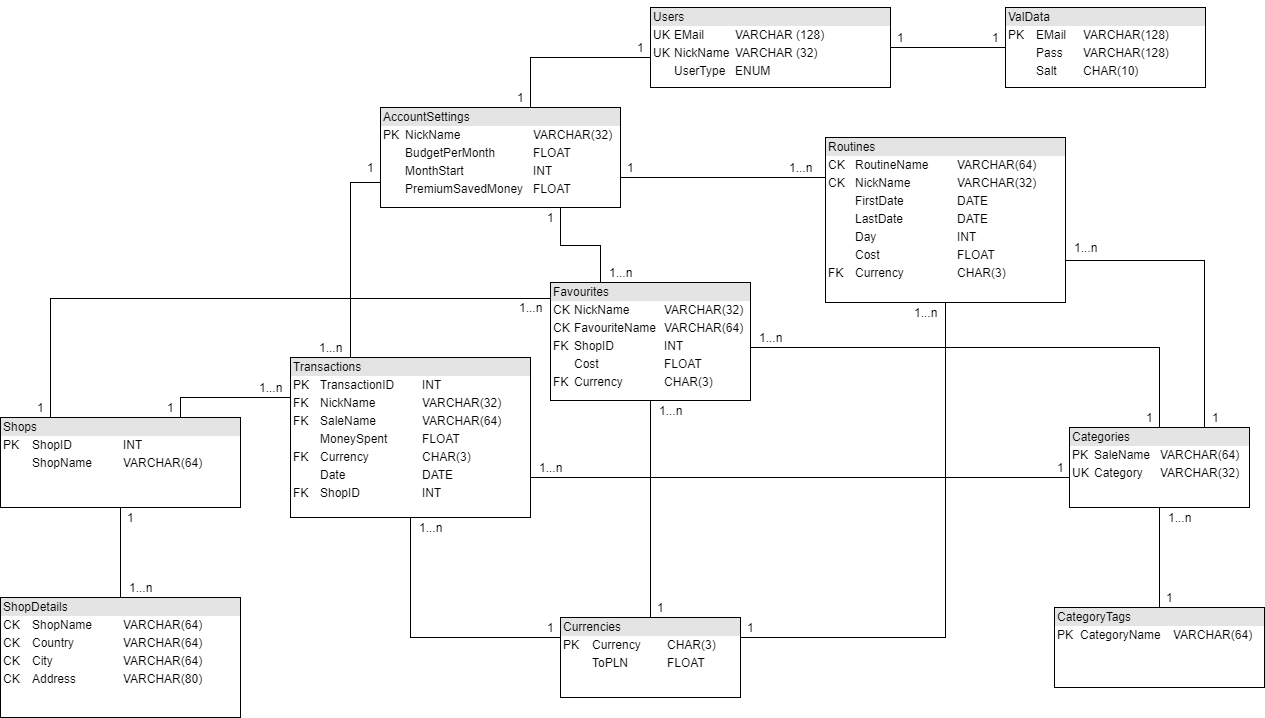
\includegraphics[width=18cm]{Project.png} 
    \end{center}
    
    \section{Legenda do diagramu UML}
    PK - Primary Key - Klucz główny
    \\FK - Foreign Key - Klucz obcy
    \\CK - Composite Key - Klucz łączony
    \\U - Unique - Wartość unikalna
    \\Users - Przechowuje dane użytkowników
    \begin{itemize}
    \item EMail - adres e-mail
    \item NickName - nazwa użytkownika
    \item UserType - rodzaj użytkownika: Podstawowy, Premium, Admin
    \end{itemize}
    ValData - Przechowuje dane uwierzytelnienia użytkowników
    \begin{itemize}
    \item EMail - adres e-mail
    \item Pass - hash od hasła użytkownika
    \item Salt - sól dołączana przy hashowaniu hasła
    \end{itemize}
    AccountSettings - Przechowuje dane o ustawieniach konta
    \begin{itemize}
    \item NickName - nazwa użytkownika
    \item BudgetPerMonth - dostępny miesięczny budżet
    \item MonthStart - dzień miesiąca, rozpoczynający okres rozliczeniowy
    \item SavedMoney(Premium) - Oszczędności, usługa dostępna przy koncie Premium
    \end{itemize}
    Transactions - Przechowuje rekordy transakcji użytkowników
    \begin{itemize}
    \item TransactionID - numer transakcji
    \item NickName - nazwa użytkownika
    \item SaleName - nazwa produktu, usługi
    \item MoneySpent - koszt kupna produktu, usługi
    \item Currency - waluta
    \item Date - data transakcji
    \item ShopID - numer identyfikacyjny sklepu
    \end{itemize}
    Routines (Premium) - Przechowuje dane o płatnościach stałych użytkowników Premium
    \begin{itemize}
    \item RoutineName - nazwa płatności stałej
    \item NickName - nazwa użytkownika
    \item FirstDate - data ustanowienia płatności stałej
    \item LastDate - data zakończenia płatności stałej
    \item Day - dzień miesiąca wykonania płatności stałej
    \item Cost - koszt płatności
    \item Currency - waluta
    \end{itemize}
    Favourites (Premium) - Przechowuje dane o ulubionych płatnościach użytkowników Premium
    \begin{itemize}
    \item NickName - nazwa użytkownika
    \item FavouriteName - nazwa płatności
    \item ShopID - numer identyfikacyjny sklepu
    \item Cost - koszt płatności
    \item Currency - waluta
    \end{itemize}
    Categories - Przechowuje dane o kategoriach produktów, usług podanych w transakcjach
    \begin{itemize}
    \item SaleName - nazwa płatności
    \item Category - nazwa kategorii
    \end{itemize}
    Shops - Przechowuje podstawowe dane o sklepach i miejscach świadczenia usług
    \begin{itemize}
    \item ShopID - numer identyfikacyjny sklepu
    \item ShopName - nazwa sklepu
    \end{itemize}
    ShopDetails - Przechowuje szczegółowe dane o sklepach i miejscach świadczenia usług
    \begin{itemize}
    \item ShopID - numer identyfikacyjny sklepu
    \item Country - adres sklepu; kraj
    \item City - adres sklepu; miasto
    \item Address - adres sklepu; ulica i numer
    \end{itemize}
    
    \section{Scenariusze użycia}
    Aplikacja ma duże możliwości, natomiast podane poniżej są 
przykładowe scenariusze jej użycia:
    \begin{enumerate}
    \item Użytkownik zakłada konto, ustala miesięczny budżet do 
rozdysponowania, następnie w danym miesiącu wprowadza dane o opłaconych 
usługach.
    \item Klient postanawia sprawdzić w jakim sklepie zakupił produkt po 
najniższej cenie, kiedy transakcja odbyła się ponad miesiąc wcześniej. 
Sprawdza historię płatności, ogranicza wyniki do produktu i sortuje po 
dacie.
    \item Klient zastanawia się ile miesięcznie płaci za poranną kawę, 
którą pije od czasu do czasu przed rozpoczęciem pracy, więc ustawia tę 
czynność jako ulubioną i sprawdza sumę kosztów pod koniec miesiąca.
    \item Student chce oszczędzić pewną sumę z dostępnego dla niego 
budżetu, a po paru miesiącach, wydać ją na zakup dobrej książki, więc 
włącza opcję liczenia osczędności w aplikacji.
    \item Użytkownik włącza do miesięcznych rachunków stałą płatność za 
Internet, abonament telefoniczny etc. W konkretnym ustalonym dniu, 
system odejmuje od pozostałego budżetu koszt opłacenia usługi.
    \end{enumerate}
    
    
    

\end{document}    
